\documentclass[12pt,letterpaper]{article}
\usepackage{iftex}
\ifXeTeX
  \usepackage{fontspec}
\else
  \usepackage[T1]{fontenc}
  \usepackage[utf8]{inputenc}
  \usepackage{lmodern}
\fi
\usepackage[spanish,es-nodecimaldot,es-noshorthands,es-tabla]{babel}
\usepackage{amsmath,amssymb}
\usepackage[margin=1in,headheight=15pt]{geometry}
\usepackage{graphicx}
\usepackage{booktabs}
\usepackage{longtable}
\usepackage{array}
\usepackage{float}
\usepackage{caption}
\usepackage{enumitem}
\usepackage{fancyhdr}
\usepackage[hidelinks]{hyperref}

\captionsetup{font=small,labelfont=bf}
\setlength{\parskip}{0.45em}
\setlength{\parindent}{0pt}
\renewcommand{\arraystretch}{1.15}
\newcommand{\paren}[1]{\left(#1\right)}

\pagestyle{fancy}
\fancyhf{}
\fancyhead[L]{\small Universidad Autónoma de Chihuahua}
\fancyhead[R]{\small Estadística Aplicada a la Investigación}
\fancyfoot[R]{\thepage}
\renewcommand{\headrulewidth}{0.4pt}

\begin{document}

%%%%%%%%%%%%%%%%%%%%%%%%%%%%%%%%%%%%%%%%%%%%%%%%%%%%%%%%%%%%%%%%%%%%%%%%%%%
% PORTADA
%%%%%%%%%%%%%%%%%%%%%%%%%%%%%%%%%%%%%%%%%%%%%%%%%%%%%%%%%%%%%%%%%%%%%%%%%%%
\begin{titlepage}
\vspace*{-1.6cm}
\noindent\makebox[\textwidth][c]{%
  \begin{minipage}[c]{2.9cm}\centering
\includegraphics[width=2.9cm]{logo_uach}\end{minipage}%
  \begin{minipage}[c]{14.4cm}\centering
    {\LARGE\bfseries Universidad Autónoma de Chihuahua\par}
    \vspace{0.15cm}
    {\Large\bfseries Facultad de Ingeniería\par}
    \vspace{0.1cm}
    {\large\bfseries Maestría en Ingeniería en Computación\par}
  \end{minipage}%
  \begin{minipage}[c]{2.9cm}\centering
\includegraphics[width=2.9cm]{logo_fing}\end{minipage}%
}

\vfill
\begin{center}
  {\huge\bfseries Proyecto Final 1:\\[0.2cm] Optimización de Rutas y\\[0.1cm] Eficiencia de Combustible\par}
  \vspace{1.2cm}
  {\Large\itshape Estadística Aplicada a la Investigación\par}
  {\large\textbf{\textit{Catedrático:}} \textit{Dr. José Saul De Lira Miramontes}\par}
\end{center}
\vfill

\begin{flushright}
  {\Large\textbf{\textit{Alumno:}}\par}
  {\Large\textbf{345491} González Cardoza Jonahtan\par}
\end{flushright}
\vfill

\begin{center}
  {\Large 25 de noviembre de 2026\par}
\end{center}
\end{titlepage}
\setcounter{page}{1}

%%%%%%%%%%%%%%%%%%%%%%%%%%%%%%%%%%%%%%%%%%%%%%%%%%%%%%%%%%%%%%%%%%%%%%%%%%%
\section{Introducción}

FastTrack Logistics es una empresa mediana de transporte de carga terrestre que opera en el centro del país y se especializa en entregas \emph{Just-in-Time} para el sector industrial. En el último trimestre fiscal sus costos operativos subieron 18\,\%, impulsados casi por completo por el gasto en diésel. La empresa quiere saber qué factores explican el consumo de combustible de su flota para decidir dónde actuar.

\textbf{Objetivos.}
\begin{itemize}[itemsep=0pt]
  \item Determinar si existen diferencias significativas en el consumo según el tipo de ruta (Urbana, Autopista, Montaña).
  \item Identificar la relación entre la velocidad, el peso de la carga y el consumo.
  \item Construir un modelo matemático que pronostique el consumo y responder las preguntas de negocio planteadas por la dirección.
\end{itemize}

%%%%%%%%%%%%%%%%%%%%%%%%%%%%%%%%%%%%%%%%%%%%%%%%%%%%%%%%%%%%%%%%%%%%%%%%%%%
\section{Datos y metodología}

El archivo \texttt{datos\_logistica\_transporte.csv} contiene 50 viajes, sin datos faltantes ni registros duplicados. Sus variables se describen en la Tabla~\ref{tab:variables}.

\begin{table}[H]
\centering
\caption{Variables del conjunto de datos.}
\label{tab:variables}
\begin{tabular}{lll}
\toprule
Variable & Tipo & Descripción \\
\midrule
\texttt{ID\_Viaje} & Identificador & Número del viaje (1 a 50) \\
\texttt{Tipo\_Ruta} & Categórica & Urbana (21), Autopista (15), Montaña (14) \\
\texttt{Peso\_Carga\_Ton} & Numérica & Peso de la carga, en toneladas \\
\texttt{Velocidad\_Promedio\_kmh} & Numérica & Velocidad promedio del viaje, en km/h \\
\texttt{Consumo\_Litros} & Numérica & Diésel consumido, en litros \\
\bottomrule
\end{tabular}
\end{table}

El análisis se hizo en Python (pandas, SciPy, statsmodels, scikit-learn, Matplotlib y Seaborn) en un cuaderno de Jupyter, con nivel de significancia $\alpha = 0.05$ en todas las pruebas. Se siguieron tres fases: (1)~estadística descriptiva y ANOVA de un factor, (2)~correlación de Pearson y (3)~regresión lineal múltiple. Los resultados se presentan también en un dashboard interactivo hecho con Streamlit. En el Anexo~\ref{sec:anexo} se desarrollan a mano los cálculos principales: estadística descriptiva completa, ANOVA, prueba de Tukey, correlación de Pearson y la regresión múltiple por matrices.

%%%%%%%%%%%%%%%%%%%%%%%%%%%%%%%%%%%%%%%%%%%%%%%%%%%%%%%%%%%%%%%%%%%%%%%%%%%
\section{Fase 1: análisis exploratorio y ANOVA}

\subsection{Estadística descriptiva}

En toda la flota, el consumo promedio es de 51.13~L por viaje ($s = 19.01$~L), el peso promedio de 15.41~t ($s = 7.15$~t) y la velocidad promedio de 56.56~km/h ($s = 27.05$~km/h). La Tabla~\ref{tab:desc} separa el consumo por ruta.

\begin{table}[H]
\centering
\caption{Consumo de combustible (litros) por tipo de ruta, y promedios de peso y velocidad.}
\label{tab:desc}
\small
\begin{tabular}{lcccccccc}
\toprule
 & & \multicolumn{5}{c}{Consumo (L)} & Peso & Velocidad \\
\cmidrule(lr){3-7}
Ruta & $n$ & Media & Desv. est. & Mín. & Máx. & CV (\%) & media (t) & media (km/h) \\
\midrule
Urbana    & 21 & 42.27 & 9.71  & 27.2 & 63.3 & 22.97 & 11.61 & 33.80 \\
Autopista & 15 & 41.25 & 7.21  & 27.3 & 54.9 & 17.48 & 16.15 & 94.84 \\
Montaña   & 14 & 75.01 & 17.53 & 40.3 & 90.4 & 23.37 & 20.32 & 49.70 \\
\midrule
Total     & 50 & 51.13 & 19.01 & 27.2 & 90.4 & 37.18 & 15.41 & 56.56 \\
\bottomrule
\end{tabular}
\end{table}

\begin{figure}[H]
\centering
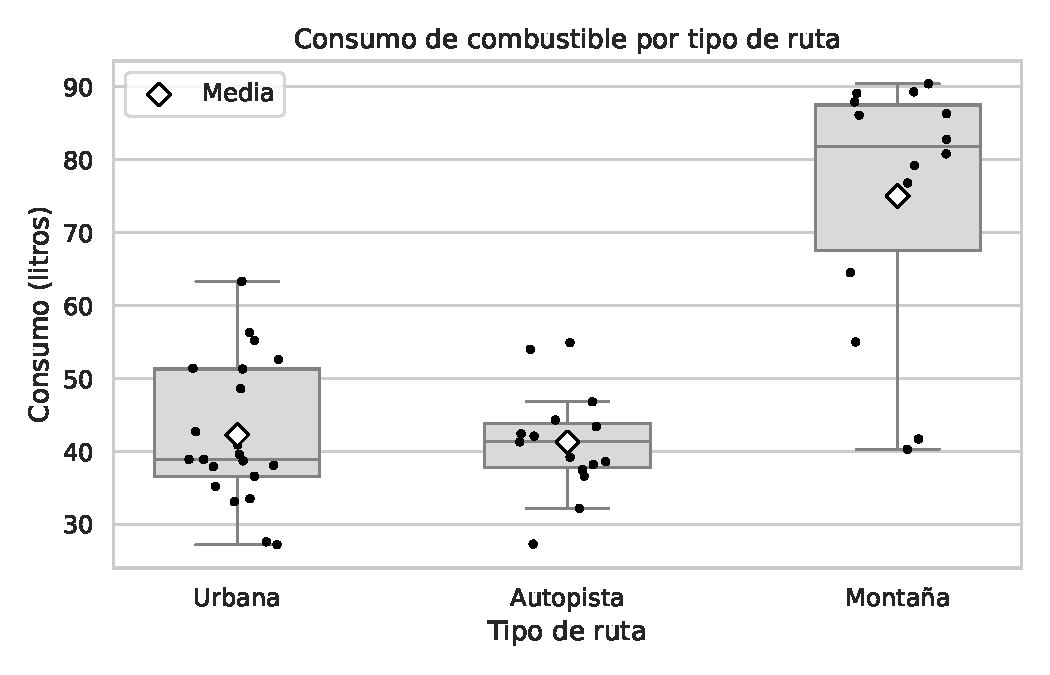
\includegraphics[width=0.72\textwidth]{figuras/fig1_boxplot_ruta.pdf}
\caption{Consumo por tipo de ruta. Cada punto es un viaje; el rombo blanco marca la media.}
\label{fig:boxplot}
\end{figure}

La ruta de montaña consume en promedio casi el doble que las otras dos (75.01~L contra 42.27 y 41.25~L), mientras que urbana y autopista se ven muy parecidas. También se observa que cada ruta tiene su propio rango de velocidad: los camiones de autopista circulan a 80--105~km/h, los de montaña a 42--60~km/h y los urbanos a 20--43~km/h. Esto será importante al interpretar la velocidad en la regresión.

\subsection{ANOVA de un factor}

Para saber si las diferencias entre rutas son reales o producto del azar se plantean las hipótesis:
$$ H_0: \mu_{\text{Urbana}} = \mu_{\text{Autopista}} = \mu_{\text{Montaña}} \qquad\qquad H_1: \text{al menos una media es diferente} $$

\begin{table}[H]
\centering
\caption{Tabla ANOVA de un factor para el consumo según el tipo de ruta.}
\label{tab:anova}
\begin{tabular}{lrrrrr}
\toprule
Fuente de variación & SC & gl & CM & $F$ & Valor $p$ \\
\midrule
Entre rutas    & 11\,099.39 & 2  & 5\,549.69 & 39.465 & $8.73 \times 10^{-11}$ \\
Dentro (error) &  6\,609.28 & 47 &    140.62 &        & \\
Total          & 17\,708.67 & 49 &           &        & \\
\bottomrule
\end{tabular}
\end{table}

El valor crítico es $F_{0.05,\,2,\,47} = 3.195$. Como $F = 39.465 > 3.195$ y el valor $p = 8.73 \times 10^{-11} < 0.05$, \textbf{se rechaza $H_0$}: el consumo medio no es igual en las tres rutas. El tamaño del efecto es
$$ \eta^2 = \frac{SC_{entre}}{SC_{total}} = \frac{11\,099.39}{17\,708.67} = 0.6268 , $$
es decir, el tipo de ruta explica el 62.7\,\% de la variación del consumo.

\textbf{Interpretación del valor $p$.} Si las tres rutas consumieran en promedio lo mismo, la probabilidad de observar diferencias tan grandes como las de esta muestra sería de aproximadamente 9 en cien mil millones. Es prácticamente imposible que la diferencia se deba al azar, así que la ruta sí influye en el consumo.

\subsection{Supuestos del ANOVA}

\begin{itemize}[itemsep=2pt]
  \item \textbf{Homogeneidad de varianzas.} Prueba de Levene: $W = 2.446$, $p = 0.098 > 0.05$. Se acepta que las varianzas son iguales.
  \item \textbf{Normalidad.} Shapiro--Wilk por grupo: Urbana $p = 0.261$, Autopista $p = 0.650$ y Montaña $p = 0.005$. La ruta de montaña no es normal porque tiene unos pocos viajes con carga ligera que consumen mucho menos que el resto (se ven abajo en la Figura~\ref{fig:boxplot}).
  \item \textbf{Confirmación no paramétrica.} Como la normalidad falla en un grupo, se aplicó también la prueba de Kruskal--Wallis, que no la supone: $H = 21.99$, $p = 1.68 \times 10^{-5}$. La conclusión es la misma, así que el resultado del ANOVA es confiable.
\end{itemize}

\subsection{Comparaciones por pares (Tukey HSD)}

El ANOVA indica que hay diferencias, pero no entre cuáles rutas. La prueba de Tukey lo aclara (Tabla~\ref{tab:tukey}).

\begin{table}[H]
\centering
\caption{Prueba de Tukey HSD ($\alpha = 0.05$).}
\label{tab:tukey}
\begin{tabular}{lrcc c}
\toprule
Comparación & Diferencia (L) & $p$ ajustado & IC 95\,\% & ¿Diferentes? \\
\midrule
Montaña -- Autopista & 33.76 & $< 0.001$ & [23.10, 44.43] & Sí \\
Montaña -- Urbana    & 32.75 & $< 0.001$ & [22.85, 42.65] & Sí \\
Urbana -- Autopista  &  1.01 & 0.965     & [$-8.69$, 10.72] & No \\
\bottomrule
\end{tabular}
\end{table}

La ruta de montaña gasta unos 33~L más por viaje que las otras dos, y esa diferencia es significativa. Urbana y autopista no son diferentes entre sí.

%%%%%%%%%%%%%%%%%%%%%%%%%%%%%%%%%%%%%%%%%%%%%%%%%%%%%%%%%%%%%%%%%%%%%%%%%%%
\section{Fase 2: análisis de correlación}

\begin{figure}[H]
\centering
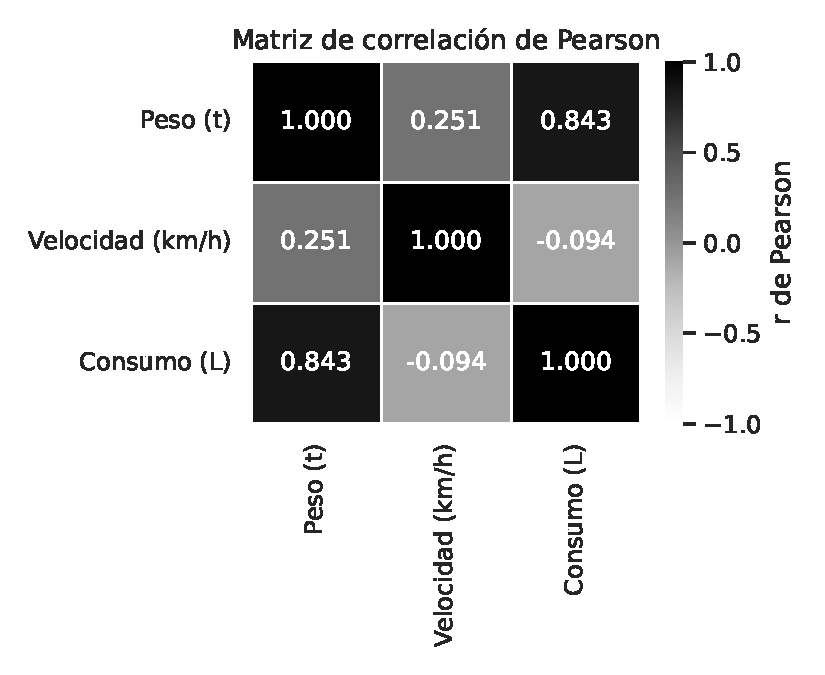
\includegraphics[width=0.55\textwidth]{figuras/fig2_correlacion.pdf}
\caption{Matriz de correlación de Pearson.}
\label{fig:corr}
\end{figure}

\begin{table}[H]
\centering
\caption{Coeficientes de Pearson y su significancia ($H_0: \rho = 0$).}
\label{tab:corr}
\begin{tabular}{lrcl}
\toprule
Par de variables & $r$ & Valor $p$ & Interpretación \\
\midrule
Peso -- Consumo       &  0.8428 & $1.64 \times 10^{-14}$ & Positiva fuerte, significativa \\
Velocidad -- Consumo  & $-0.0939$ & 0.517 & Prácticamente nula, no significativa \\
Peso -- Velocidad     &  0.2509 & 0.079 & Débil, no significativa \\
\bottomrule
\end{tabular}
\end{table}

\textbf{La variable con la relación más fuerte con el consumo es el peso de la carga} ($r = 0.843$): a mayor peso, mayor consumo. La velocidad, vista sobre toda la flota, parece no tener relación con el consumo ($r = -0.094$).

Sin embargo, la Figura~\ref{fig:disp} muestra por qué la velocidad engaña: los viajes forman tres nubes según la ruta. Los camiones más rápidos (autopista) no son los que más gastan, y los de montaña, con velocidad intermedia, son los que más consumen. Si se calcula la correlación dentro de cada ruta, el peso sigue siendo casi perfecto ($r = 0.969$ en urbana, $0.972$ en autopista y $0.996$ en montaña), mientras que la velocidad muestra relaciones positivas que van de nulas a moderadas ($r = 0.598$, $0.023$ y $0.384$). Es decir, la ruta funciona como variable de confusión y hay que incluirla en el modelo.

\begin{figure}[H]
\centering
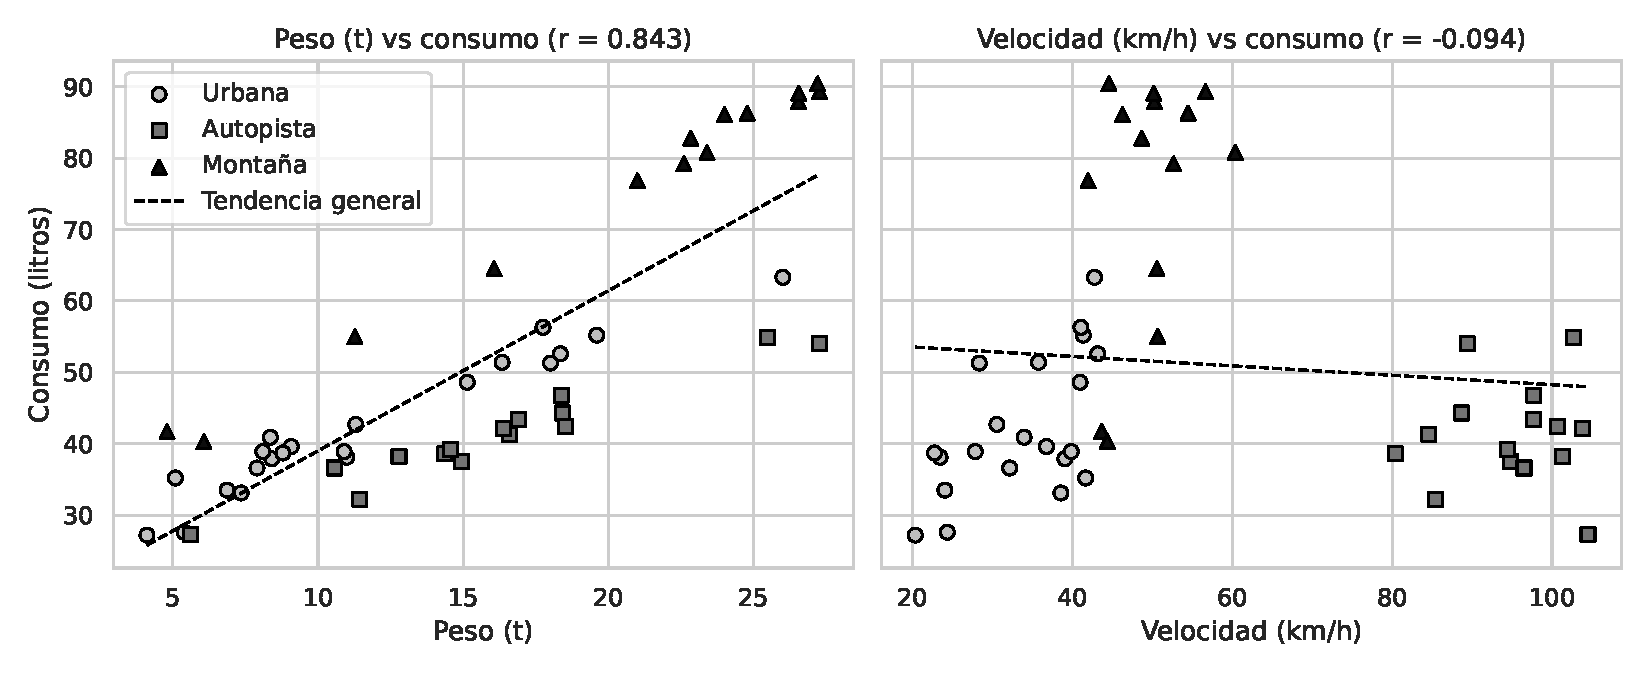
\includegraphics[width=\textwidth]{figuras/fig3_dispersion.pdf}
\caption{Peso y velocidad contra consumo. La línea punteada es la tendencia de toda la flota.}
\label{fig:disp}
\end{figure}

%%%%%%%%%%%%%%%%%%%%%%%%%%%%%%%%%%%%%%%%%%%%%%%%%%%%%%%%%%%%%%%%%%%%%%%%%%%
\section{Fase 3: regresión lineal múltiple}

Se ajustaron tres modelos por mínimos cuadrados. El Modelo~1 es el que pide el caso; los Modelos 2 y 3 agregan el tipo de ruta para corregir el efecto de confusión detectado en la fase anterior.

\subsection{Modelo 1: peso y velocidad}\label{sec:m1}

$$ \widehat{Consumo} = b_0 + b_1\,Peso + b_2\,Velocidad $$

\begin{table}[H]
\centering
\caption{Coeficientes del Modelo 1.}
\label{tab:m1}
\begin{tabular}{lrrrcc}
\toprule
Término & Coeficiente & Error est. & $t$ & Valor $p$ & IC 95\,\% \\
\midrule
Intercepto ($b_0$) & 26.1794 & 3.4618 & 7.562  & $1.15 \times 10^{-9}$  & [19.215, 33.144] \\
Peso ($b_1$)       &  2.4600 & 0.1748 & 14.071 & $1.81 \times 10^{-18}$ & [2.108, 2.812] \\
Velocidad ($b_2$)  & $-0.2290$ & 0.0462 & $-4.959$ & $9.67 \times 10^{-6}$ & [$-0.322$, $-0.136$] \\
\bottomrule
\end{tabular}
\end{table}

$$ \boxed{\widehat{Consumo} = 26.1794 + 2.4600\,Peso - 0.2290\,Velocidad} $$

$R^2 = 0.8098$, $R^2_{aj} = 0.8017$, $F = 100.08$ ($p = 1.15 \times 10^{-17}$). Los tres coeficientes son significativos ($p < 0.05$). Cada tonelada adicional aumenta el consumo en 2.46~L, y cada km/h adicional lo \emph{reduciría} en 0.23~L.

Ese signo negativo de la velocidad no tiene sentido físico: es consecuencia de la confusión con la ruta. Los camiones rápidos son los de autopista, que es la ruta que menos gasta, así que el modelo le atribuye a la velocidad el ahorro que en realidad se debe a la ruta. Además, los residuos de este modelo no son normales (Shapiro--Wilk $p = 0.033$).

\subsection{Modelo 2: se agrega el tipo de ruta}

Se agregan dos variables ficticias, \emph{Urbana} y \emph{Montaña} (valen 1 si el viaje es de esa ruta y 0 si no), con autopista como referencia.

\begin{table}[H]
\centering
\caption{Coeficientes del Modelo 2 (referencia: Autopista).}
\label{tab:m2}
\begin{tabular}{lrrrcc}
\toprule
Término & Coeficiente & Error est. & $t$ & Valor $p$ & IC 95\,\% \\
\midrule
Intercepto    &  1.0277 & 6.2832 & 0.164  & 0.871                  & [$-11.628$, 13.683] \\
Peso          &  1.7792 & 0.0765 & 23.266 & $1.01 \times 10^{-26}$ & [1.625, 1.933] \\
Velocidad     &  0.1212 & 0.0683 & 1.774  & 0.083                  & [$-0.016$, 0.259] \\
Ruta Urbana   & 16.4832 & 4.2188 & 3.907  & $3.11 \times 10^{-4}$  & [7.986, 24.980] \\
Ruta Montaña  & 31.8149 & 3.3995 & 9.359  & $3.98 \times 10^{-12}$ & [24.968, 38.662] \\
\bottomrule
\end{tabular}
\end{table}

$$ \widehat{Consumo} = 1.0277 + 1.7792\,Peso + 0.1212\,Velocidad + 16.4832\,Urbana + 31.8149\,Montaña $$

$R^2 = 0.9748$, $R^2_{aj} = 0.9726$, $F = 435.52$ ($p = 2.42 \times 10^{-35}$). Al controlar la ruta:
\begin{itemize}[itemsep=2pt]
  \item El \textbf{peso} sigue siendo muy significativo: 1.78~L más por cada tonelada.
  \item La \textbf{velocidad} cambia de signo a positivo (0.12~L por km/h, lo que sí tiene sentido físico) y deja de ser significativa ($p = 0.083 > 0.05$).
  \item Con el mismo peso y velocidad, un viaje de \textbf{montaña} gasta 31.8~L más que uno de autopista, y uno urbano 16.5~L más (este último porque en ciudad se va a velocidades muy bajas, con arranques y paradas).
  \item El intercepto no es significativo, lo cual no es problema: no tiene interpretación práctica (sería un camión sin carga a 0~km/h).
\end{itemize}

Los residuos ya son normales (Shapiro--Wilk $p = 0.205$) y no muestran patrón (Figura~\ref{fig:resid}). Los VIF de velocidad (16.9) y de las variables de ruta (21.9 y 11.8) son altos porque la velocidad depende casi por completo de la ruta; por eso su coeficiente tiene un error estándar grande. El peso no tiene ese problema (VIF = 1.5).

\subsection{Modelo 3: el efecto del peso depende de la ruta}

Para saber si la carga pesada cuesta más en alguna ruta, se agregó la interacción Peso~$\times$~Ruta. El término Peso~$\times$~Montaña es significativo ($b = 0.928$, $p = 9.1 \times 10^{-10}$), mientras que Peso~$\times$~Urbana no lo es ($p = 0.057$). Este modelo alcanza $R^2 = 0.9910$ y en él la velocidad tiene un efecto positivo pequeño (0.11~L por km/h, $p = 0.013$). Las pendientes del peso en cada ruta se resumen en la Tabla~\ref{tab:pendientes}.

\begin{table}[H]
\centering
\caption{Litros adicionales por cada tonelada de carga, según la ruta (Modelo 3).}
\label{tab:pendientes}
\begin{tabular}{lcc}
\toprule
Ruta & L por tonelada & Relativo a autopista \\
\midrule
Autopista & 1.307 & 1.00 \\
Urbana    & 1.552 & 1.19 \\
Montaña   & 2.234 & 1.71 \\
\bottomrule
\end{tabular}
\end{table}

\begin{figure}[H]
\centering
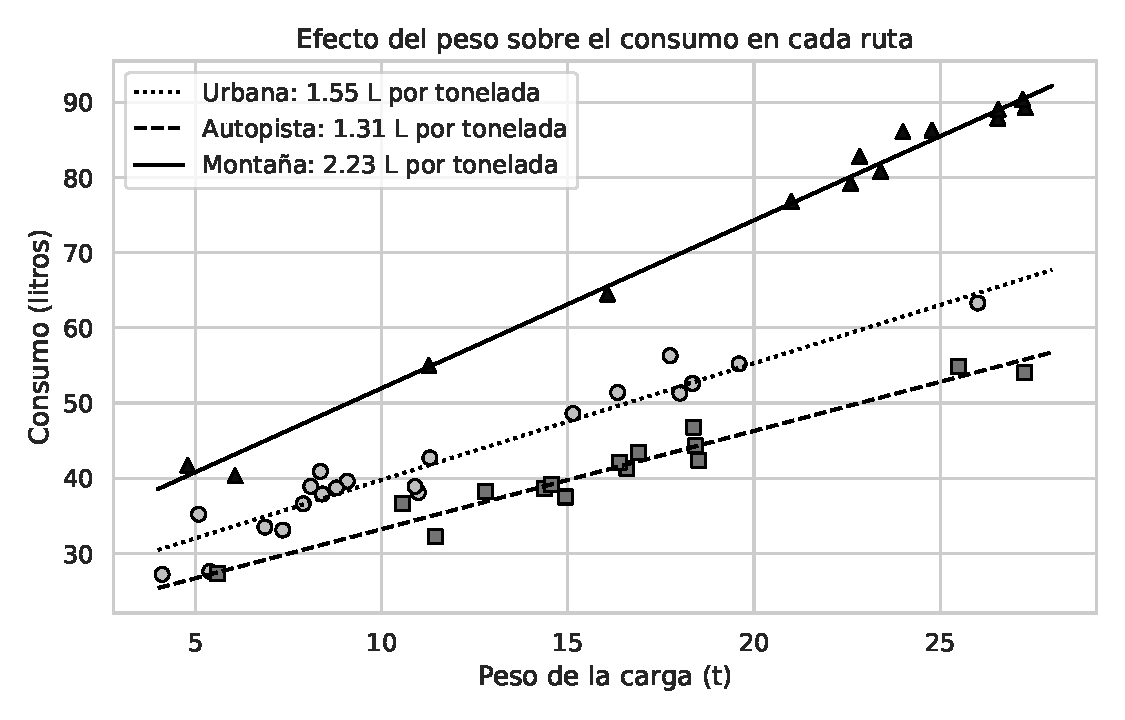
\includegraphics[width=0.75\textwidth]{figuras/fig4_peso_por_ruta.pdf}
\caption{Efecto del peso sobre el consumo en cada ruta (rectas del Modelo 3 a la velocidad media de cada ruta).}
\label{fig:pendientes}
\end{figure}

\subsection{Métricas de rendimiento}

Además de las métricas sobre los mismos datos, se hizo \textbf{validación cruzada de 5 bloques}: cada viaje se predice con un modelo que no lo usó para ajustarse, lo que mide qué tan bien pronostica el modelo viajes nuevos.

\begin{table}[H]
\centering
\caption{Comparación de los modelos. RMSE y MAE en litros; VC = validación cruzada de 5 bloques.}
\label{tab:metricas}
\begin{tabular}{lccccccc}
\toprule
Modelo & $R^2$ & $R^2_{aj}$ & RMSE & MAE & $R^2$ VC & RMSE VC & AIC \\
\midrule
1: Peso + Velocidad   & 0.8098 & 0.8017 & 8.207 & 6.995 & 0.7809 & 8.810 & 358.4 \\
2: + Ruta             & 0.9748 & 0.9726 & 2.986 & 2.391 & 0.9657 & 3.487 & 261.3 \\
3: + Peso $\times$ Ruta & 0.9910 & 0.9897 & 1.788 & 1.469 & 0.9870 & 2.146 & 214.0 \\
\bottomrule
\end{tabular}
\end{table}

Agregar la ruta reduce el error típico de pronóstico de unos 8.8~L a 3.5~L por viaje, y la interacción lo baja a 2.1~L. Las métricas de validación cruzada son casi iguales a las del ajuste, así que los modelos no están sobreajustados.

\begin{figure}[H]
\centering
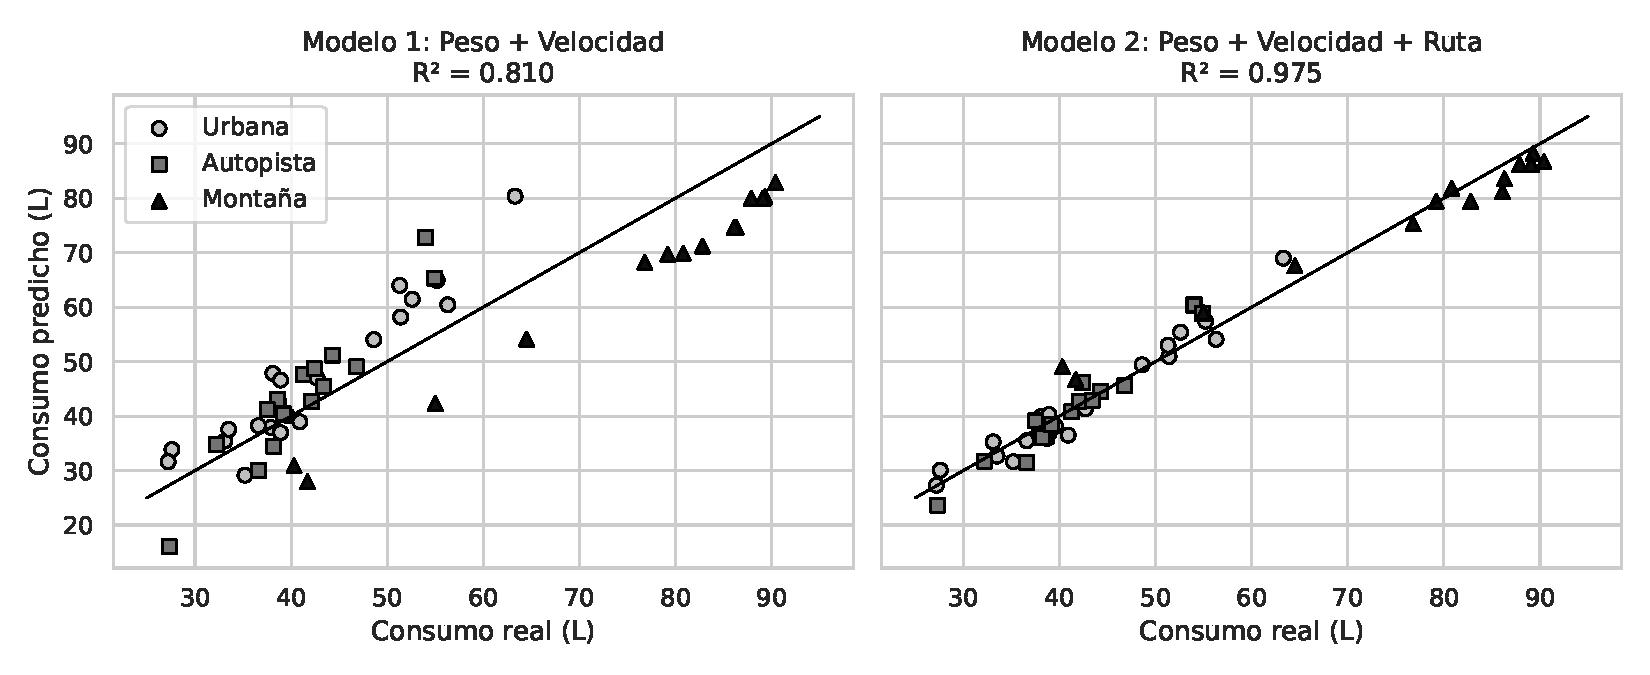
\includegraphics[width=\textwidth]{figuras/fig5_real_vs_predicho.pdf}
\caption{Consumo real contra predicho. Entre más cerca de la diagonal, mejor el pronóstico.}
\label{fig:realpred}
\end{figure}

\begin{figure}[H]
\centering
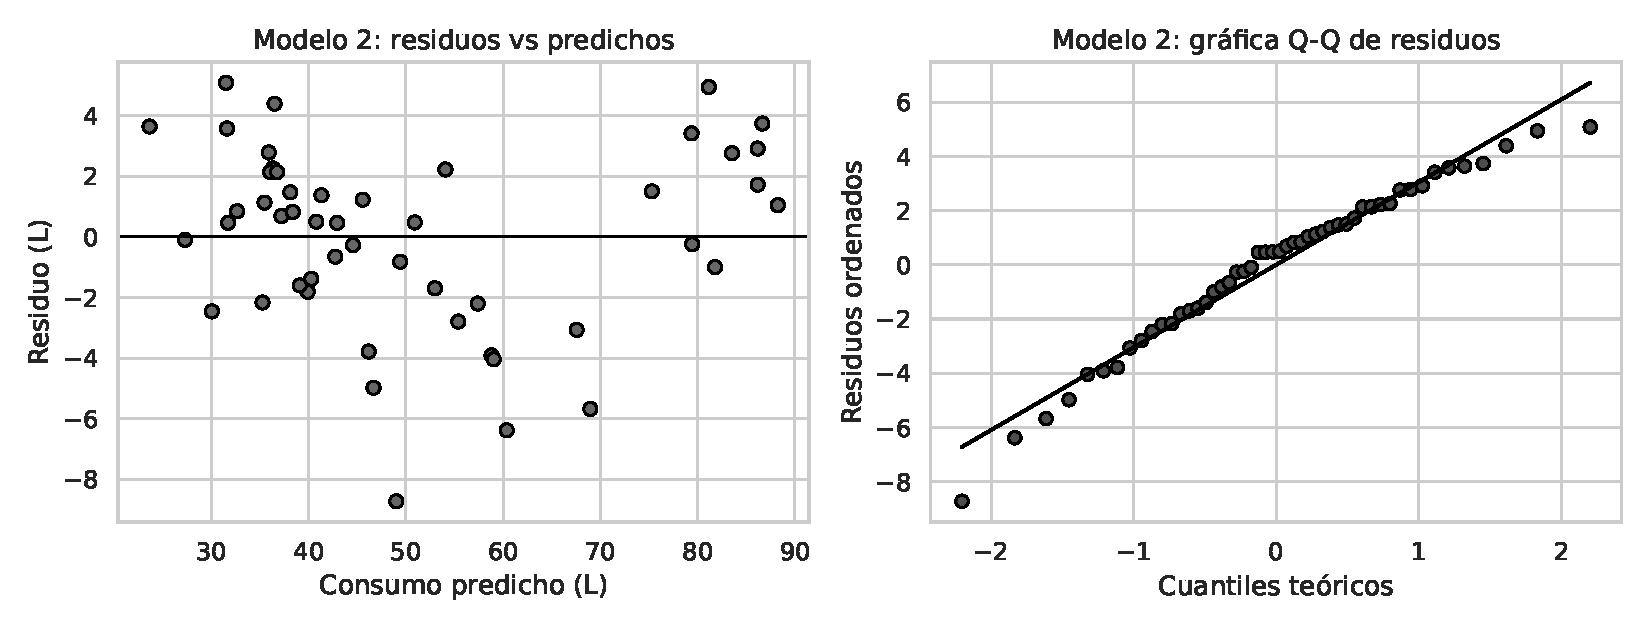
\includegraphics[width=\textwidth]{figuras/fig6_residuos.pdf}
\caption{Diagnóstico de residuos del Modelo 2: sin patrón y aproximadamente normales.}
\label{fig:resid}
\end{figure}

\subsection{¿Qué pesa más: la velocidad o la carga?}

Como el peso (toneladas) y la velocidad (km/h) tienen unidades distintas, sus coeficientes se comparan estandarizados ($\beta = b \cdot s_x / s_y$): cuántas desviaciones estándar cambia el consumo cuando la variable sube una desviación estándar.

\begin{table}[H]
\centering
\caption{Coeficientes normales y estandarizados del peso y la velocidad.}
\label{tab:beta}
\begin{tabular}{lccccc}
\toprule
Modelo & $b$ Peso (L/t) & $b$ Velocidad (L por km/h) & $\beta$ Peso & $\beta$ Velocidad & $p$ Velocidad \\
\midrule
Modelo 1 & 2.4600 & $-0.2290$ & 0.925 & $-0.326$ & $< 0.001$ \\
Modelo 2 & 1.7792 & 0.1212 & 0.669 & 0.172 & 0.083 \\
\bottomrule
\end{tabular}
\end{table}

En el Modelo 2 el efecto del peso es casi cuatro veces el de la velocidad. En términos prácticos, reducir la carga 5~t ahorra $5 \times 1.7792 = 8.90$~L por viaje, mientras que bajar la velocidad 10~km/h ahorra solo $10 \times 0.1212 = 1.21$~L, y ese efecto ni siquiera es significativo.

%%%%%%%%%%%%%%%%%%%%%%%%%%%%%%%%%%%%%%%%%%%%%%%%%%%%%%%%%%%%%%%%%%%%%%%%%%%
\section{Pronóstico: camión con 15 toneladas a 80 km/h}

\textbf{Con el Modelo 1} (la ecuación que pide el caso):
$$ \widehat{Consumo} = 26.1794 + 2.4600(15) - 0.2290(80) = 26.1794 + 36.9000 - 18.3200 = \boxed{44.76 \text{ L}} $$
(con los coeficientes sin redondear el resultado es 44.76~L). Intervalo de confianza del 95\,\% para el consumo medio: [41.48, 48.03]~L. Intervalo de predicción del 95\,\% para un viaje individual: [27.42, 62.10]~L.

\textbf{Con el Modelo 2}, el pronóstico depende de la ruta. Una velocidad promedio de 80~km/h solo se observa en autopista (rango de 80.4 a 104.5~km/h), así que ese es el escenario realista:
$$ \widehat{Consumo} = 1.0277 + 1.7792(15) + 0.1212(80) = 1.0277 + 26.6880 + 9.6960 = \boxed{37.41 \text{ L}} $$
con intervalo de predicción del 95\,\% de [30.57, 44.26]~L, mucho más angosto que el del Modelo 1. Para comparar, el mismo camión daría 53.90~L en ruta urbana y 69.23~L en montaña, pero esas dos cifras son extrapolaciones, porque en esas rutas nunca se observó una velocidad de 80~km/h.

%%%%%%%%%%%%%%%%%%%%%%%%%%%%%%%%%%%%%%%%%%%%%%%%%%%%%%%%%%%%%%%%%%%%%%%%%%%
\section{Toma de decisiones}

\begin{enumerate}[itemsep=6pt]
  \item \textbf{¿Debería la empresa evitar ciertas rutas para cargas pesadas?}\\
  Sí, la \textbf{montaña}. Además de gastar más de base, en montaña cada tonelada adicional cuesta 2.23~L, contra 1.31~L en autopista y 1.55~L en ciudad (Tabla~\ref{tab:pendientes}); la diferencia es significativa ($p < 0.001$). Por ejemplo, llevar 10~t extra por montaña cuesta unos 9~L más que llevarlas por autopista. Las cargas pesadas conviene mandarlas por autopista cuando exista la opción, o dividirlas en viajes más ligeros si la ruta de montaña es obligatoria.

  \item \textbf{¿En qué tipo de ruta se gasta más combustible y la diferencia es significativa?}\\
  En \textbf{montaña}: 75.01~L promedio por viaje, contra 42.27~L en urbana y 41.25~L en autopista. El ANOVA confirma que la diferencia es estadísticamente significativa ($F = 39.47$, $p = 8.7 \times 10^{-11}$), y la ruta explica el 62.7\,\% de la variación del consumo. Según Tukey, montaña difiere de las otras dos rutas, pero urbana y autopista no difieren entre sí.

  \item \textbf{¿Enfocarse en controlar la velocidad o en reducir el peso de la carga?}\\
  En \textbf{reducir el peso}. Es la variable con mayor correlación con el consumo ($r = 0.843$), es significativa en todos los modelos y su efecto estandarizado es casi cuatro veces el de la velocidad. Bajar 5~t ahorra unos 8.9~L por viaje; bajar 10~km/h, solo 1.2~L. El coeficiente negativo de la velocidad en el Modelo~1 no debe usarse para decidir (sugeriría acelerar para ahorrar), porque es un efecto de la confusión con la ruta.

  \item \textbf{Pronóstico para un camión con 15 toneladas a 80 km/h.}\\
  Con la ecuación del Modelo 1: \textbf{44.76~L}. Si el viaje es por autopista (la única ruta donde se observan 80~km/h), el Modelo 2, que es más preciso, pronostica \textbf{37.41~L}.
\end{enumerate}

%%%%%%%%%%%%%%%%%%%%%%%%%%%%%%%%%%%%%%%%%%%%%%%%%%%%%%%%%%%%%%%%%%%%%%%%%%%
\section{Conclusiones}

\begin{itemize}[itemsep=3pt]
  \item El consumo de diésel depende sobre todo de \textbf{dos factores: el tipo de ruta y el peso de la carga}. Juntos explican el 97.5\,\% de la variación del consumo.
  \item La ruta de montaña es la más cara y además castiga más las cargas pesadas. Urbana y autopista consumen lo mismo en promedio.
  \item La velocidad tiene un efecto pequeño. Analizada sola, su relación con el consumo es engañosa, porque cada ruta tiene su propio rango de velocidades; este es un ejemplo de por qué la correlación simple no basta y hay que controlar las variables de confusión.
  \item Para el pronóstico se recomienda el Modelo 2 (o el 3, si se quiere máxima precisión) en lugar del Modelo 1: su error típico es de unos 3.5~L por viaje contra 8.8~L, y sus coeficientes tienen sentido físico.
  \item \textbf{Recomendación para la empresa:} planear la asignación de carga por ruta, priorizando la autopista para los envíos pesados, y controlar el peso por viaje, que es la palanca con más impacto. Limitar la velocidad puede tener otras ventajas (seguridad, desgaste), pero el ahorro de combustible que se puede esperar de ello es pequeño.
  \item \textbf{Limitaciones:} la muestra es de 50 viajes y no incluye otras variables que influyen en el consumo (pendiente exacta, tráfico, clima, estado del camión, estilo de manejo). Los pronósticos fuera de los rangos observados, como 80~km/h en ciudad, deben tomarse con cautela.
\end{itemize}

%%%%%%%%%%%%%%%%%%%%%%%%%%%%%%%%%%%%%%%%%%%%%%%%%%%%%%%%%%%%%%%%%%%%%%%%%%%
\section{Entregables}

\begin{enumerate}[itemsep=2pt]
  \item \textbf{Dataset:} carpeta \texttt{dataset/}, con el archivo original \texttt{datos\_logistica\_transporte1.csv} y \texttt{datos\_logistica\_transporte.csv} (los mismos 50 viajes convertidos a codificación UTF-8).
  \item \textbf{Reporte:} este documento, en la carpeta \texttt{reporte/} junto con su código \LaTeX, las figuras y los logos.
  \item \textbf{Modelos predictivos con métricas:} Modelos 1, 2 y 3, con $R^2$, $R^2$ ajustado, RMSE, MAE, AIC y validación cruzada (Tabla~\ref{tab:metricas}).
  \item \textbf{Código:} cuaderno de Jupyter \texttt{Proyecto\_final\_analisis.ipynb}, en la carpeta principal, con todo el análisis. Al ejecutarlo vuelve a generar el dataset limpio y las figuras del reporte.
  \item \textbf{Dashboard:} aplicación de Streamlit \texttt{app\_dashboard.py}, en la carpeta principal, que se ejecuta desde esa carpeta con \texttt{streamlit run app\_dashboard.py} (las librerías necesarias están en \texttt{requirements.txt}). Tiene una pestaña de presentación y pestañas de descriptivos, ANOVA, correlación, regresión, un simulador de consumo y las respuestas de decisión (Figuras~\ref{fig:dash1} y~\ref{fig:dash2}).
\end{enumerate}

\begin{figure}[H]
\centering
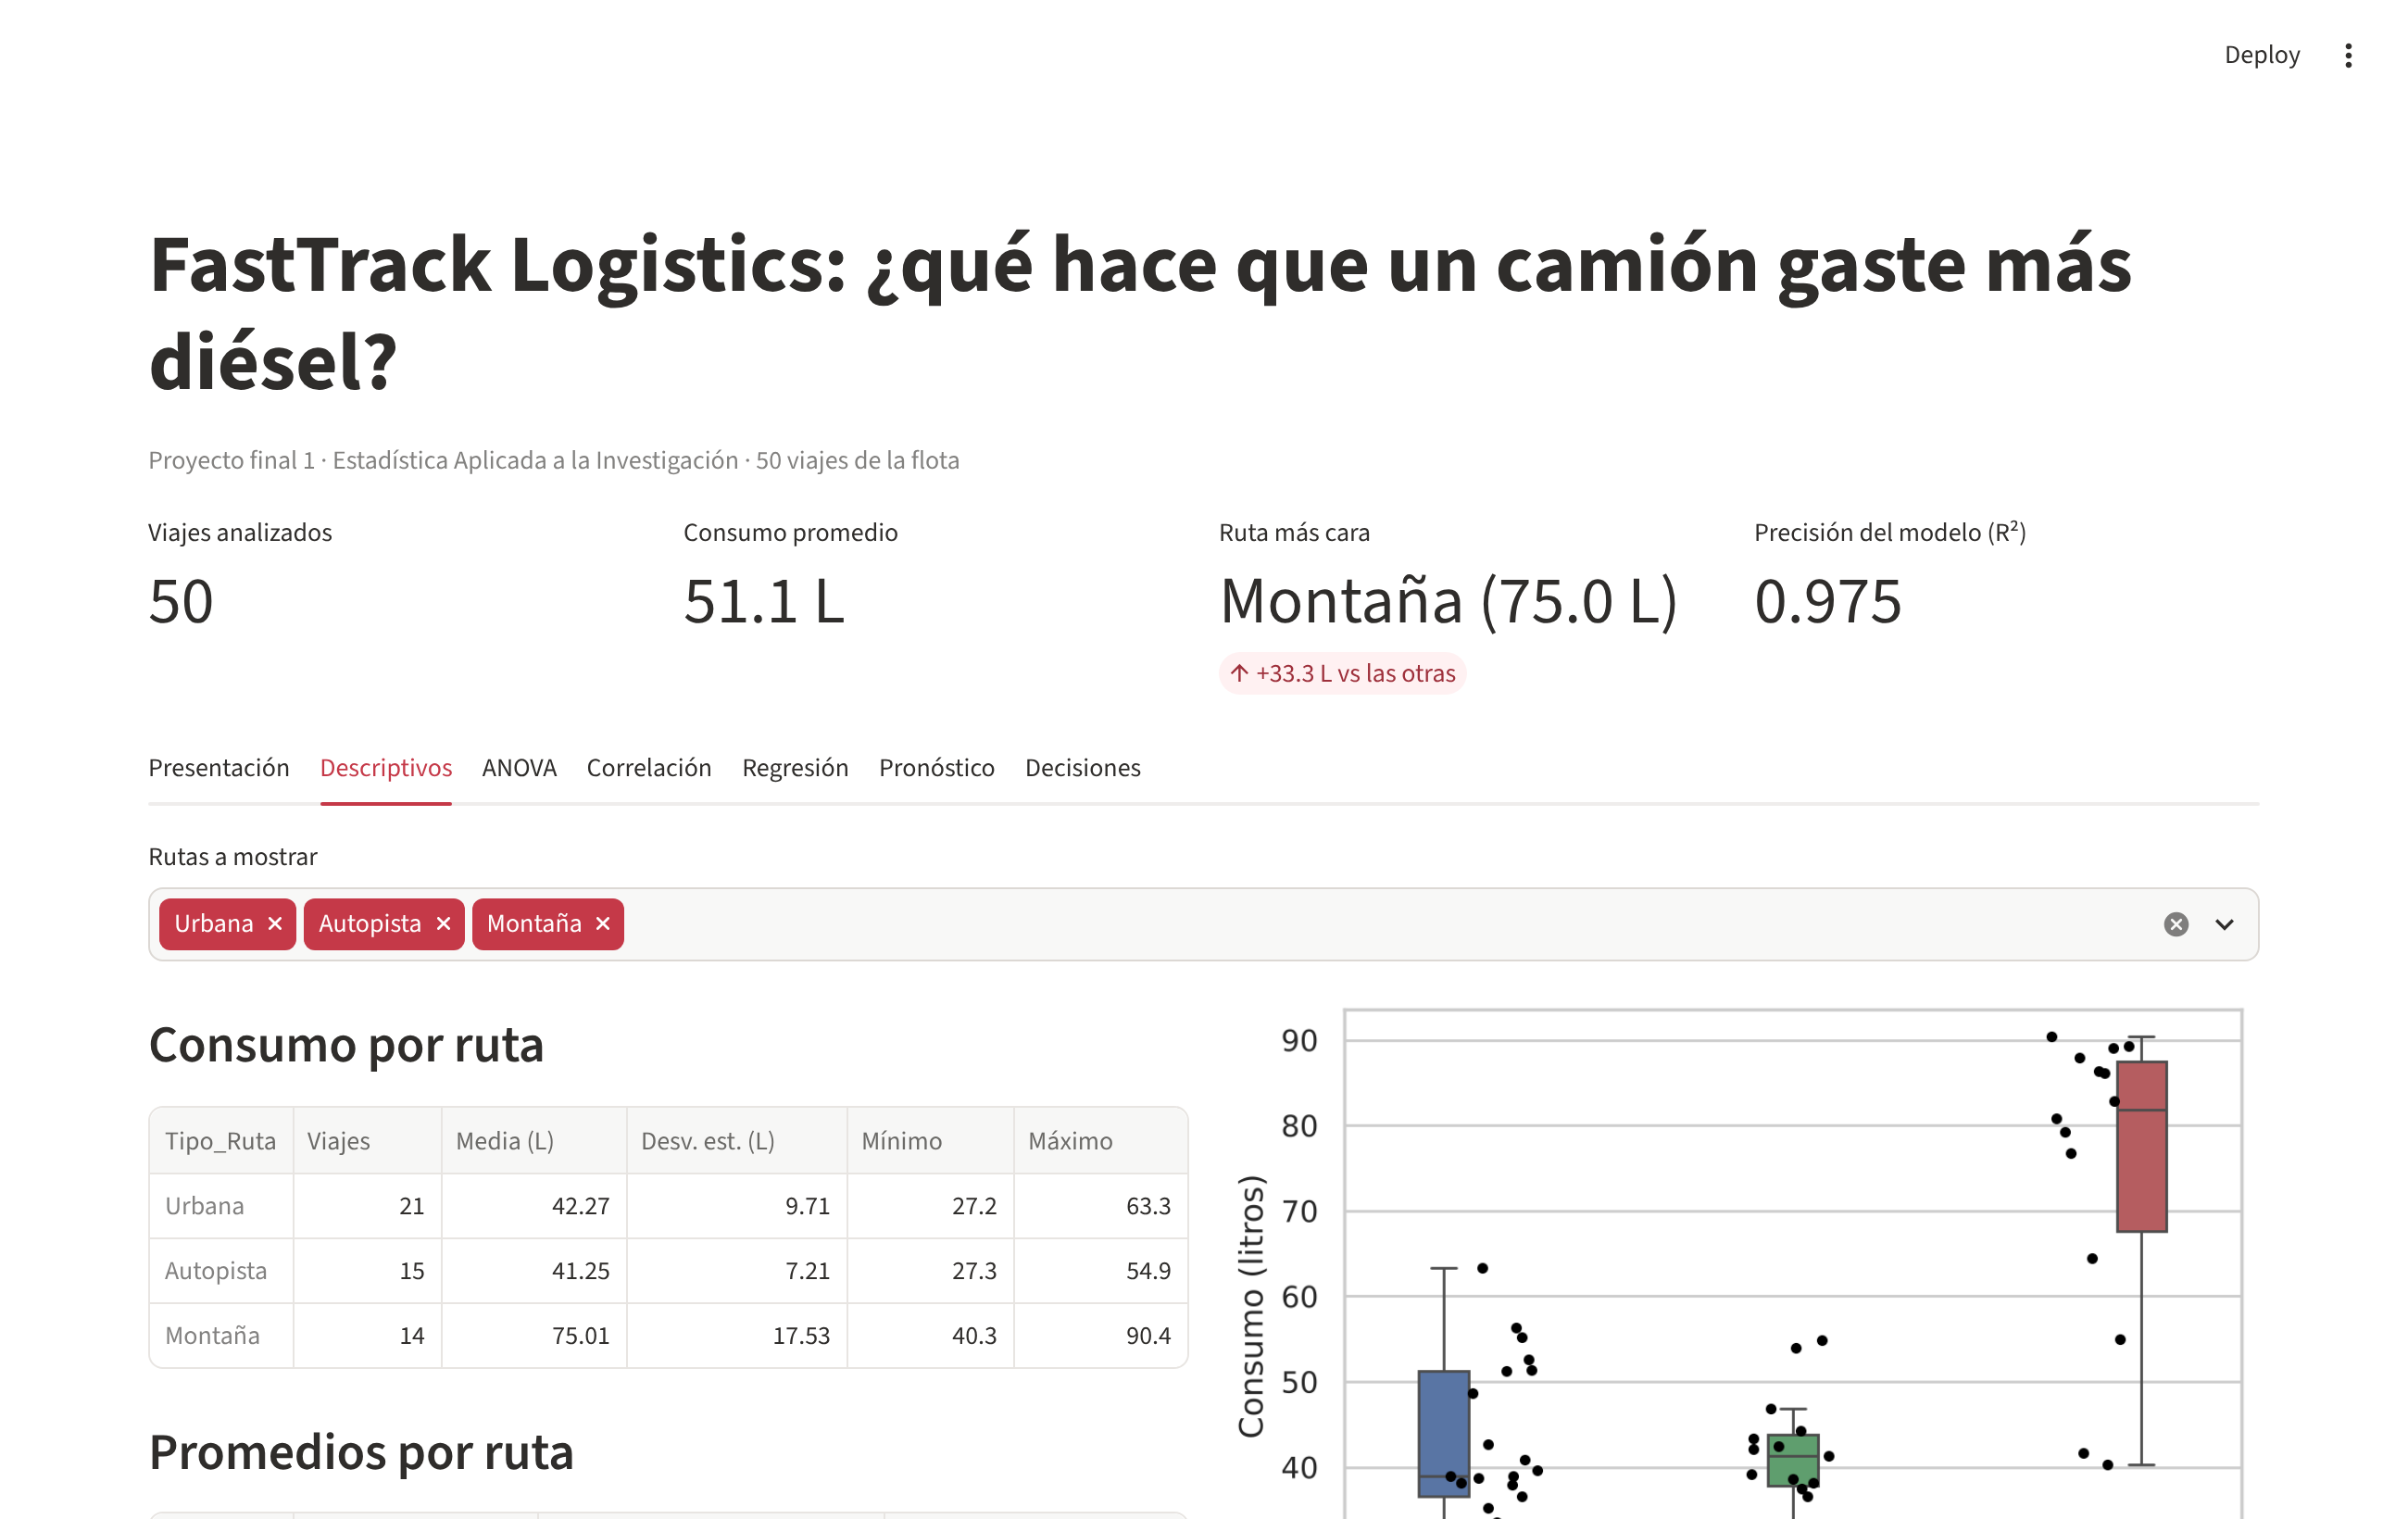
\includegraphics[width=\textwidth]{figuras/dashboard_descriptivos.png}
\caption{Dashboard en Streamlit: indicadores generales y pestaña de descriptivos.}
\label{fig:dash1}
\end{figure}

\begin{figure}[H]
\centering
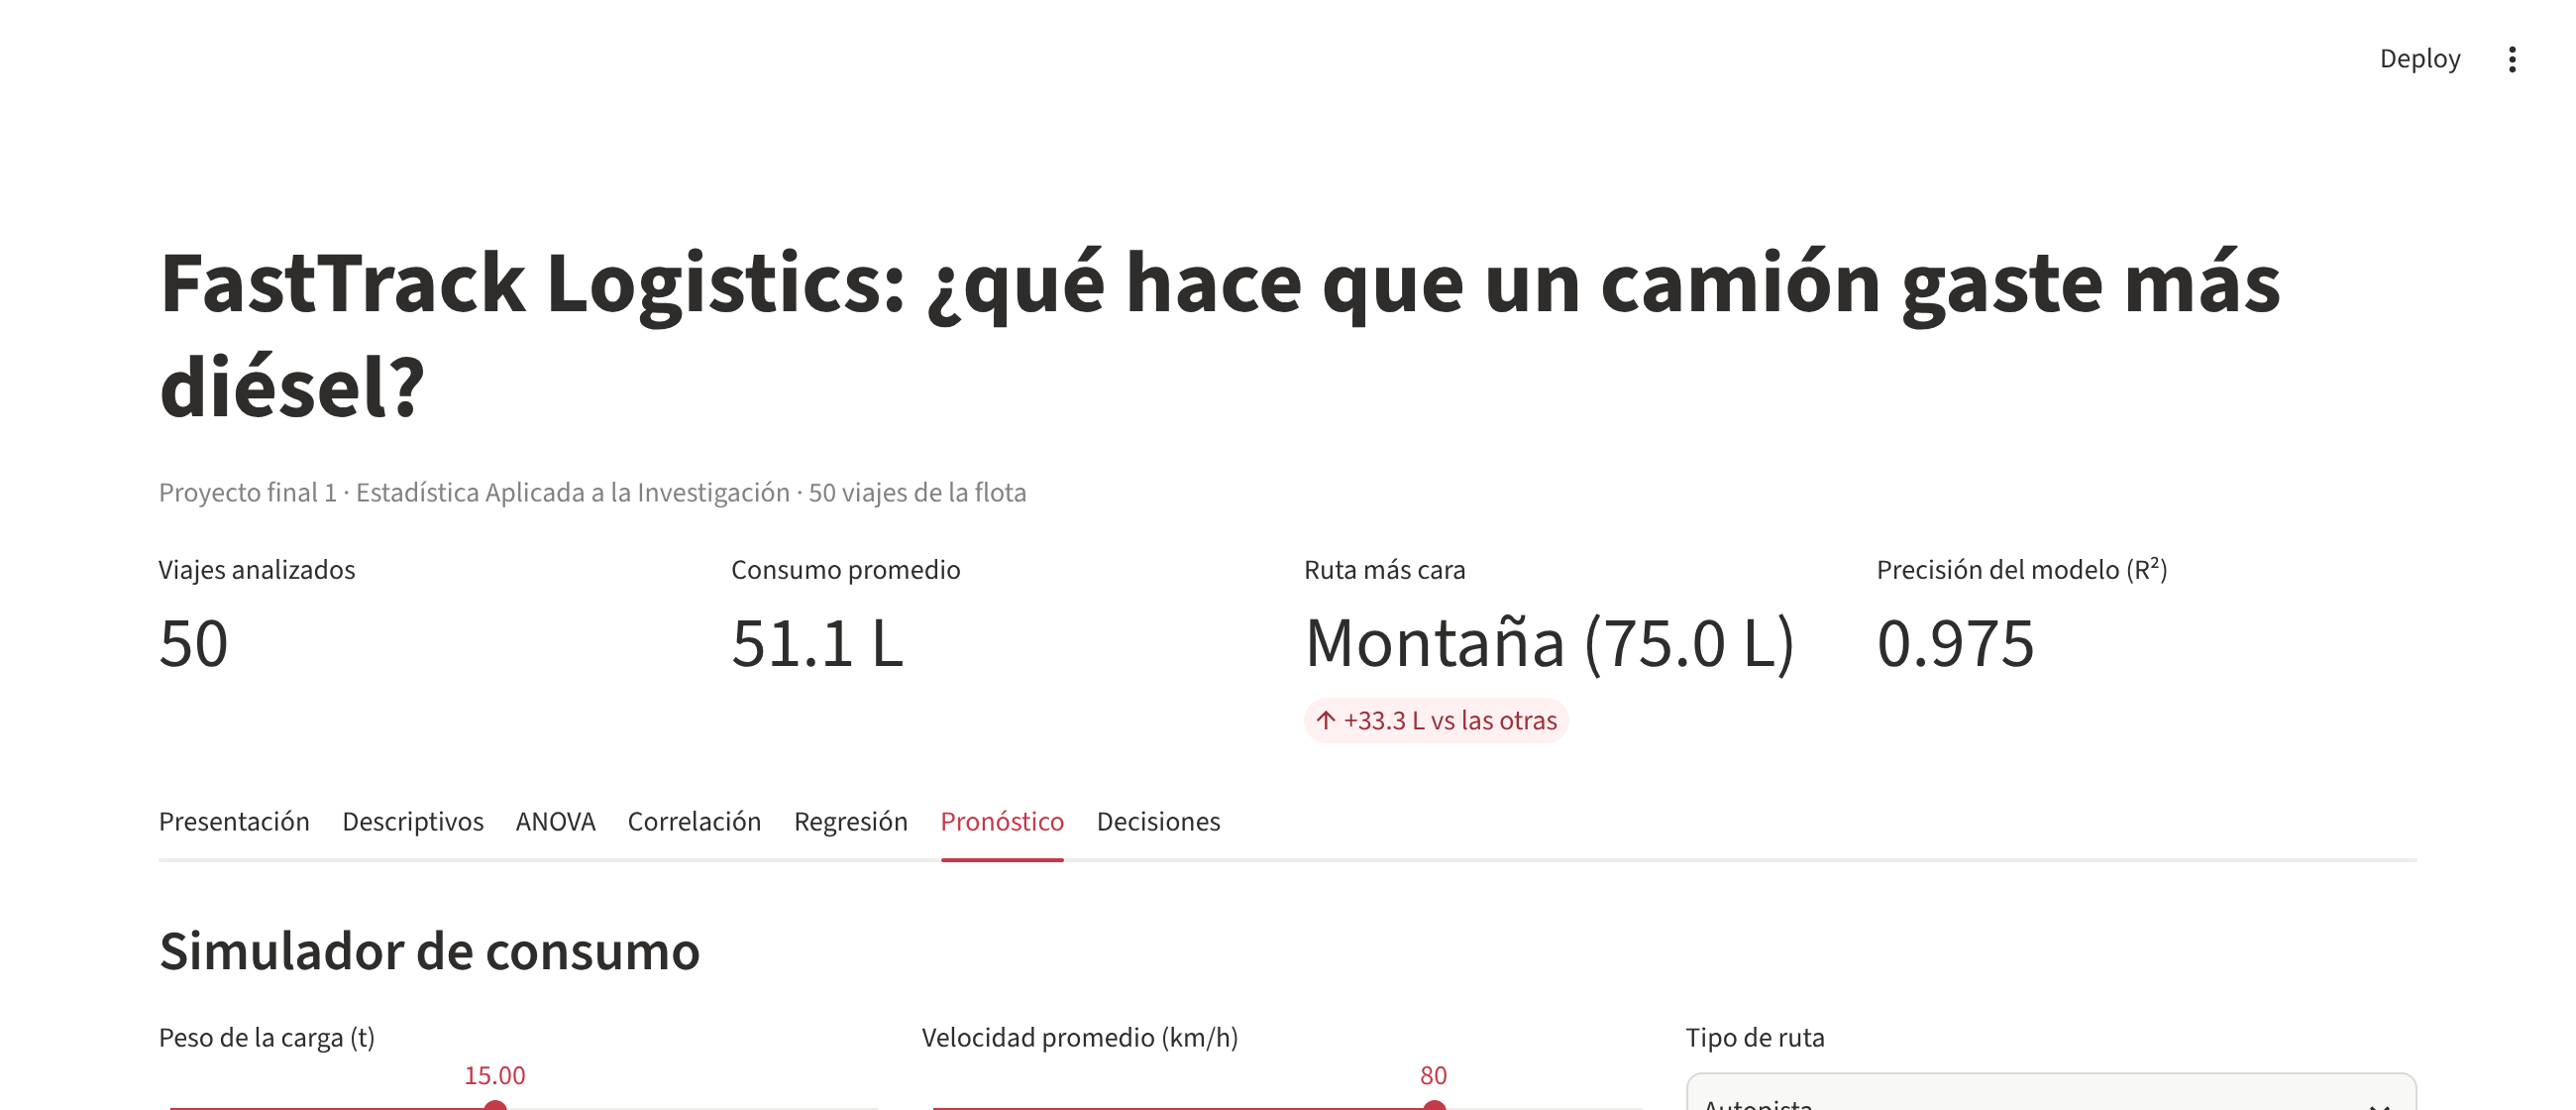
\includegraphics[width=\textwidth]{figuras/dashboard_pronostico.png}
\caption{Dashboard en Streamlit: simulador de consumo con el caso de 15~t a 80~km/h.}
\label{fig:dash2}
\end{figure}


%%%%%%%%%%%%%%%%%%%%%%%%%%%%%%%%%%%%%%%%%%%%%%%%%%%%%%%%%%%%%%%%%%%%%%%%%%%
\clearpage
\appendix
\section{Cálculos a mano}\label{sec:anexo}

En este anexo se desarrollan paso a paso los cálculos principales del análisis, con las fórmulas y la sustitución de los valores. Todos los resultados coinciden con los obtenidos en Python. Se usa $n_j$ para el número de viajes de la ruta $j$, $N = 50$ para el total y $k = 3$ para el número de rutas.

\subsection{Estadística descriptiva completa por ruta}

Fórmulas utilizadas, para una muestra $x_1, \dots, x_n$:
$$ \bar{x} = \frac{\sum x_i}{n} $$
$$ s^2 = \frac{\sum \paren{x_i - \bar{x}}^2}{n - 1} $$
$$ s = \sqrt{s^2} $$
$$ R = x_{max} - x_{min} $$
$$ CV = \frac{s}{\bar{x}} \times 100 $$
La mediana es el valor central de los datos ordenados (o el promedio de los dos centrales si $n$ es par) y la moda es el valor que más se repite.

\begin{table}[H]
\centering
\caption{Estadística descriptiva: Peso de la carga (t).}
\small\setlength{\tabcolsep}{4.5pt}
\begin{tabular}{lcrrcrrrrr}
\toprule
Ruta & $n$ & Media & Mediana & Moda & Varianza & Desv. est. & Mín. & Máx. & Rango \\
\midrule
Urbana & 21 & 11.61 & 9.08 & Sin moda & 33.52 & 5.79 & 4.11 & 26.01 & 21.90 \\
Autopista & 15 & 16.15 & 16.38 & Sin moda & 29.32 & 5.41 & 5.60 & 27.27 & 21.67 \\
Montaña & 14 & 20.32 & 23.12 & Sin moda & 59.42 & 7.71 & 4.80 & 27.28 & 22.48 \\
\midrule
Total & 50 & 15.41 & 15.61 & Sin moda & 51.05 & 7.15 & 4.11 & 27.28 & 23.17 \\
\bottomrule
\end{tabular}
\end{table}

\begin{table}[H]
\centering
\caption{Estadística descriptiva: Velocidad promedio (km/h).}
\small\setlength{\tabcolsep}{4.5pt}
\begin{tabular}{lcrrcrrrrr}
\toprule
Ruta & $n$ & Media & Mediana & Moda & Varianza & Desv. est. & Mín. & Máx. & Rango \\
\midrule
Urbana & 21 & 33.80 & 35.80 & Sin moda & 58.10 & 7.62 & 20.40 & 43.20 & 22.80 \\
Autopista & 15 & 94.84 & 96.50 & 97.7 (2) & 57.18 & 7.56 & 80.40 & 104.50 & 24.10 \\
Montaña & 14 & 49.70 & 50.25 & Sin moda & 27.68 & 5.26 & 42.00 & 60.40 & 18.40 \\
\midrule
Total & 50 & 56.56 & 45.45 & 97.7 (2) & 731.52 & 27.05 & 20.40 & 104.50 & 84.10 \\
\bottomrule
\end{tabular}
\end{table}

\begin{table}[H]
\centering
\caption{Estadística descriptiva: Consumo de combustible (L).}
\small\setlength{\tabcolsep}{4.5pt}
\begin{tabular}{lcrrcrrrrr}
\toprule
Ruta & $n$ & Media & Mediana & Moda & Varianza & Desv. est. & Mín. & Máx. & Rango \\
\midrule
Urbana & 21 & 42.27 & 38.90 & 38.9 (2) & 94.23 & 9.71 & 27.20 & 63.30 & 36.10 \\
Autopista & 15 & 41.25 & 41.30 & Sin moda & 52.03 & 7.21 & 27.30 & 54.90 & 27.60 \\
Montaña & 14 & 75.01 & 81.80 & Sin moda & 307.41 & 17.53 & 40.30 & 90.40 & 50.10 \\
\midrule
Total & 50 & 51.13 & 42.55 & 36.6, 38.9 (2) & 361.40 & 19.01 & 27.20 & 90.40 & 63.20 \\
\bottomrule
\end{tabular}
\end{table}

La moda se acompaña de su frecuencia entre paréntesis. Las velocidades de cada ruta casi no se traslapan, y la ruta de montaña concentra las cargas más pesadas y la mayor dispersión del consumo.

\subsection{ANOVA de un factor del consumo}

\textbf{Paso 1. Totales y medias por ruta.}

\begin{table}[H]
\centering
\caption{Datos resumidos del consumo por ruta.}
\begin{tabular}{lcccc}
\toprule
Ruta & $n_j$ & $T_j = \sum x_{ij}$ & $\bar{x}_j = T_j / n_j$ & $s_j^2$ \\
\midrule
Urbana & 21 & 887.6 & 42.2667 & 94.2273 \\
Autopista & 15 & 618.8 & 41.2533 & 52.0270 \\
Montaña & 14 & 1\,050.2 & 75.0143 & 307.4121 \\
\midrule
Total & 50 & 2\,556.6 & 51.1320 & \\
\bottomrule
\end{tabular}
\end{table}

La media general es $\bar{\bar{x}} = \dfrac{2\,556.6}{50} = 51.1320$ L.

\textbf{Paso 2. Suma de cuadrados entre rutas.}
$$ SC_{entre} = \sum_{j=1}^{k} n_j \paren{\bar{x}_j - \bar{\bar{x}}}^2 $$
$$ SC_{entre} = 21\paren{42.2667 - 51.1320}^2 + 15\paren{41.2533 - 51.1320}^2 + 14\paren{75.0143 - 51.1320}^2 $$
$$ SC_{entre} = 1650.4768 + 1463.8208 + 7985.0900 = 11\,099.3877 $$

\textbf{Paso 3. Suma de cuadrados dentro de las rutas.} Como $\sum_i (x_{ij} - \bar{x}_j)^2 = (n_j - 1)s_j^2$:
$$ SC_{dentro} = \sum_{j=1}^{k} (n_j - 1)\,s_j^2 = (20)(94.2273) + (14)(52.0270) + (13)(307.4121) $$
$$ SC_{dentro} = 1884.5467 + 728.3773 + 3996.3571 = 6\,609.2811 $$

\textbf{Paso 4. Comprobación con la suma de cuadrados total.} Con $\sum x^2 = 148\,432.74$:
$$ SC_{total} = \sum x_{ij}^2 - \frac{T^2}{N} = 148\,432.74 - \frac{(2\,556.6)^2}{50} = 17\,708.6688 $$
$$ SC_{entre} + SC_{dentro} = 11\,099.3877 + 6\,609.2811 = 17\,708.6688 \;\checkmark $$

\textbf{Paso 5. Grados de libertad, cuadrados medios y estadístico $F$.}
$$ gl_{entre} = k - 1 = 2 \qquad gl_{dentro} = N - k = 47 \qquad gl_{total} = N - 1 = 49 $$
$$ CM_{entre} = \frac{SC_{entre}}{gl_{entre}} = \frac{11\,099.3877}{2} = 5\,549.6938 $$
$$ CM_{dentro} = \frac{SC_{dentro}}{gl_{dentro}} = \frac{6\,609.2811}{47} = 140.6230 $$
$$ F = \frac{CM_{entre}}{CM_{dentro}} = \frac{5\,549.6938}{140.6230} = 39.4650 $$

\textbf{Paso 6. Decisión.} El valor crítico es $F_{0.05,\,2,\,47} = 3.1951$. Como $39.4650 > 3.1951$ (valor $p = 8.735 \times 10^{-11}$), se rechaza $H_0$. El tamaño del efecto es
$$ \eta^2 = \frac{SC_{entre}}{SC_{total}} = \frac{11\,099.3877}{17\,708.6688} = 0.6268 $$


\subsection{Prueba de Tukey a mano (Tukey--Kramer)}

Como los grupos tienen distinto tamaño, se usa la versión de Tukey--Kramer. Con $q_{0.05;\,3;\,47} = 3.4226$ (tabla del rango estudentizado, $k = 3$ y $gl = 47$), la diferencia mínima significativa de cada par es:
$$ HSD_{ij} = q \sqrt{\frac{CM_{dentro}}{2}\paren{\frac{1}{n_i} + \frac{1}{n_j}}} $$

$$ HSD_{\text{Montaña--Autopista}} = 3.4226\sqrt{\frac{140.6230}{2}\paren{\frac{1}{14} + \frac{1}{15}}} = 10.6648 $$
$$ HSD_{\text{Montaña--Urbana}} = 3.4226\sqrt{\frac{140.6230}{2}\paren{\frac{1}{14} + \frac{1}{21}}} = 9.9021 $$
$$ HSD_{\text{Urbana--Autopista}} = 3.4226\sqrt{\frac{140.6230}{2}\paren{\frac{1}{21} + \frac{1}{15}}} = 9.7020 $$

\begin{table}[H]
\centering
\caption{Comparación de las diferencias de medias contra la HSD de cada par.}
\begin{tabular}{lcccc}
\toprule
Par & $|\bar{x}_i - \bar{x}_j|$ & $HSD_{ij}$ & ¿$|\bar{x}_i - \bar{x}_j| > HSD$? & Conclusión \\
\midrule
Montaña -- Autopista & 33.7610 & 10.6648 & Sí & Diferentes \\
Montaña -- Urbana & 32.7476 & 9.9021 & Sí & Diferentes \\
Urbana -- Autopista & 1.0133 & 9.7020 & No & Iguales \\
\bottomrule
\end{tabular}
\end{table}

\subsection{ANOVA del peso y de la velocidad por ruta}

Con el mismo procedimiento se comparan el peso y la velocidad entre rutas. Sirve para entender por qué la ruta influye tanto en el consumo.

\begin{table}[H]
\centering
\caption{ANOVA de un factor de las tres variables según la ruta ($F_{0.05,\,2,\,47} = 3.1951$).}
\small\setlength{\tabcolsep}{4pt}
\begin{tabular}{lrrrrcc}
\toprule
Variable & $SC_{entre}$ & $SC_{dentro}$ & $F$ & Valor $p$ & $\eta^2$ & Levene $p$ \\
\midrule
Consumo (L) & 11\,099.3877 & 6\,609.2811 & 39.4650 & $8.735 \times 10^{-11}$ & 0.6268 & 0.0976 \\
Peso (t) & 648.1895 & 1\,853.3885 & 8.2187 & $8.693 \times 10^{-4}$ & 0.2591 & 0.6810 \\
Velocidad (km/h) & 33\,522.1323 & 2\,322.3455 & 339.2131 & $1.176 \times 10^{-28}$ & 0.9352 & 0.1915 \\
\bottomrule
\end{tabular}
\end{table}

En las tres variables se rechaza $H_0$ ($F > 3.1951$) y se cumple la homogeneidad de varianzas (Levene $p > 0.05$). El peso también cambia según la ruta: según Tukey, montaña lleva en promedio 8.70~t más que urbana ($p = 0.0006$), y las demás parejas no difieren. La velocidad está separada casi por completo por ruta ($\eta^2 = 0.94$). Esto confirma que parte del mayor consumo de montaña se debe a que ahí van las cargas más pesadas; el Modelo 2 separa ambos efectos y muestra que, aun con el mismo peso, montaña gasta 31.8~L más que autopista.


\subsection{Correlación de Pearson a mano}

Las sumas de los 50 viajes (columnas $\Sigma$ de la Tabla~\ref{tab:sumas}) son:
$$ \sum x_1 = 770.48 \qquad \sum x_2 = 2\,828.1 \qquad \sum y = 2\,556.6 $$
$$ \sum x_1^2 = 14\,374.3666 \qquad \sum x_2^2 = 195\,807.47 \qquad \sum y^2 = 148\,432.74 $$
$$ \sum x_1 x_2 = 45\,955.687 \qquad \sum x_1 y = 45\,005.833 \qquad \sum x_2 y = 142\,241.30 $$
donde $x_1$ es el peso, $x_2$ la velocidad y $y$ el consumo. Las sumas de cuadrados y de productos centradas son:
$$ S_{ab} = \sum ab - \frac{\sum a \sum b}{n} $$
$$ S_{11} = 14\,374.3666 - \frac{(770.48)^2}{50} = 2\,501.5780 $$
$$ S_{22} = 195\,807.47 - \frac{(2\,828.1)^2}{50} = 35\,844.4778 $$
$$ S_{yy} = 148\,432.74 - \frac{(2\,556.6)^2}{50} = 17\,708.6688 $$
$$ S_{12} = 45\,955.687 - \frac{(770.48)(2\,828.1)}{50} = 2\,375.7972 $$
$$ S_{1y} = 45\,005.833 - \frac{(770.48)(2\,556.6)}{50} = 5\,609.6496 $$
$$ S_{2y} = 142\,241.30 - \frac{(2\,828.1)(2\,556.6)}{50} = -2\,365.1092 $$

El coeficiente de Pearson es $r_{ab} = \dfrac{S_{ab}}{\sqrt{S_{aa} S_{bb}}}$:
$$ r_{x_1 y} = \frac{5\,609.6496}{\sqrt{(2\,501.5780)(17\,708.6688)}} = 0.8428 $$
$$ r_{x_2 y} = \frac{-2\,365.1092}{\sqrt{(35\,844.4778)(17\,708.6688)}} = -0.0939 $$
$$ r_{x_1 x_2} = \frac{2\,375.7972}{\sqrt{(2\,501.5780)(35\,844.4778)}} = 0.2509 $$

Para probar si cada correlación es significativa ($H_0: \rho = 0$) se usa $t = \dfrac{r\sqrt{n - 2}}{\sqrt{1 - r^2}}$ con $gl = 48$ y valor crítico $t_{0.025,\,48} = \pm 2.0106$:

$$ t_{x_1 y} = \frac{0.8428\sqrt{48}}{\sqrt{1 - (0.8428)^2}} = 10.8497 \;\Rightarrow\; \text{significativa} $$
$$ t_{x_2 y} = \frac{-0.0939\sqrt{48}}{\sqrt{1 - (-0.0939)^2}} = -0.6533 \;\Rightarrow\; \text{no significativa} $$
$$ t_{x_1 x_2} = \frac{0.2509\sqrt{48}}{\sqrt{1 - (0.2509)^2}} = 1.7957 \;\Rightarrow\; \text{no significativa} $$

\subsection{Regresión lineal múltiple por matrices (Modelo 1)}

El modelo $\hat{y} = b_0 + b_1 x_1 + b_2 x_2$ se resuelve por mínimos cuadrados con
$$ \mathbf{b} = (X^{\prime}X)^{-1} X^{\prime}\mathbf{y} $$
\textbf{Paso 1. Tabla de sumas.} Se calculan los cuadrados y productos de cada viaje.

{\footnotesize
\setlength{\tabcolsep}{4pt}
\begin{longtable}{|c||r|r|r||r|r|r|r|r|}
\caption{Cálculos por viaje para la regresión ($x_1$ = peso, $x_2$ = velocidad, $y$ = consumo).}\label{tab:sumas}\\
\hline
$i$ & $x_1$ & $x_2$ & $y$ & $x_1^2$ & $x_2^2$ & $x_1 x_2$ & $x_1 y$ & $x_2 y$ \\
\hline\hline
\endfirsthead
\hline
$i$ & $x_1$ & $x_2$ & $y$ & $x_1^2$ & $x_2^2$ & $x_1 x_2$ & $x_1 y$ & $x_2 y$ \\
\hline\hline
\endhead
\hline
\endfoot
1 & 27.27 & 89.4 & 54.0 & 743.6529 & 7\,992.36 & 2\,437.938 & 1\,472.580 & 4\,827.60 \\
2 & 22.60 & 52.7 & 79.2 & 510.7600 & 2\,777.29 & 1\,191.020 & 1\,789.920 & 4\,173.84 \\
3 & 26.55 & 50.3 & 87.9 & 704.9025 & 2\,530.09 & 1\,335.465 & 2\,333.745 & 4\,421.37 \\
4 & 25.48 & 102.7 & 54.9 & 649.2304 & 10\,547.29 & 2\,616.796 & 1\,398.852 & 5\,638.23 \\
5 & 18.35 & 43.2 & 52.6 & 336.7225 & 1\,866.24 & 792.720 & 965.210 & 2\,272.32 \\
6 & 19.60 & 41.4 & 55.2 & 384.1600 & 1\,713.96 & 811.440 & 1\,081.920 & 2\,285.28 \\
7 & 5.39 & 24.4 & 27.6 & 29.0521 & 595.36 & 131.516 & 148.764 & 673.44 \\
8 & 24.78 & 54.5 & 86.3 & 614.0484 & 2\,970.25 & 1\,350.510 & 2\,138.514 & 4\,703.35 \\
9 & 18.43 & 88.7 & 44.3 & 339.6649 & 7\,867.69 & 1\,634.741 & 816.449 & 3\,929.41 \\
10 & 21.00 & 42.0 & 76.8 & 441.0000 & 1\,764.00 & 882.000 & 1\,612.800 & 3\,225.60 \\
11 & 17.75 & 41.1 & 56.3 & 315.0625 & 1\,689.21 & 729.525 & 999.325 & 2\,313.93 \\
12 & 27.28 & 56.7 & 89.3 & 744.1984 & 3\,214.89 & 1\,546.776 & 2\,436.104 & 5\,063.31 \\
13 & 24.00 & 46.3 & 86.1 & 576.0000 & 2\,143.69 & 1\,111.200 & 2\,066.400 & 3\,986.43 \\
14 & 9.08 & 36.8 & 39.6 & 82.4464 & 1\,354.24 & 334.144 & 359.568 & 1\,457.28 \\
15 & 8.36 & 34.0 & 40.9 & 69.8896 & 1\,156.00 & 284.240 & 341.924 & 1\,390.60 \\
16 & 8.41 & 39.1 & 37.9 & 70.7281 & 1\,528.81 & 328.831 & 318.739 & 1\,481.89 \\
17 & 11.30 & 30.6 & 42.7 & 127.6900 & 936.36 & 345.780 & 482.510 & 1\,306.62 \\
18 & 16.59 & 84.6 & 41.3 & 275.2281 & 7\,157.16 & 1\,403.514 & 685.167 & 3\,493.98 \\
19 & 14.37 & 80.4 & 38.6 & 206.4969 & 6\,464.16 & 1\,155.348 & 554.682 & 3\,103.44 \\
20 & 10.99 & 23.5 & 38.1 & 120.7801 & 552.25 & 258.265 & 418.719 & 895.35 \\
21 & 18.52 & 100.7 & 42.4 & 342.9904 & 10\,140.49 & 1\,864.964 & 785.248 & 4\,269.68 \\
22 & 7.35 & 38.6 & 33.1 & 54.0225 & 1\,489.96 & 283.710 & 243.285 & 1\,277.66 \\
23 & 10.90 & 27.9 & 38.9 & 118.8100 & 778.41 & 304.110 & 424.010 & 1\,085.31 \\
24 & 12.79 & 101.3 & 38.2 & 163.5841 & 10\,261.69 & 1\,295.627 & 488.578 & 3\,869.66 \\
25 & 14.94 & 94.8 & 37.5 & 223.2036 & 8\,987.04 & 1\,416.312 & 560.250 & 3\,555.00 \\
26 & 22.84 & 48.7 & 82.8 & 521.6656 & 2\,371.69 & 1\,112.308 & 1\,891.152 & 4\,032.36 \\
27 & 8.79 & 22.8 & 38.7 & 77.2641 & 519.84 & 200.412 & 340.173 & 882.36 \\
28 & 16.34 & 35.8 & 51.4 & 266.9956 & 1\,281.64 & 584.972 & 839.876 & 1\,840.12 \\
29 & 18.01 & 28.4 & 51.3 & 324.3601 & 806.56 & 511.484 & 923.913 & 1\,456.92 \\
30 & 4.11 & 20.4 & 27.2 & 16.8921 & 416.16 & 83.844 & 111.792 & 554.88 \\
31 & 18.38 & 97.7 & 46.8 & 337.8244 & 9\,545.29 & 1\,795.726 & 860.184 & 4\,572.36 \\
32 & 8.10 & 39.9 & 38.9 & 65.6100 & 1\,592.01 & 323.190 & 315.090 & 1\,552.11 \\
33 & 5.60 & 104.5 & 27.3 & 31.3600 & 10\,920.25 & 585.200 & 152.880 & 2\,852.85 \\
34 & 26.56 & 50.2 & 89.1 & 705.4336 & 2\,520.04 & 1\,333.312 & 2\,366.496 & 4\,472.82 \\
35 & 27.21 & 44.6 & 90.4 & 740.3841 & 1\,989.16 & 1\,213.566 & 2\,459.784 & 4\,031.84 \\
36 & 23.40 & 60.4 & 80.8 & 547.5600 & 3\,648.16 & 1\,413.360 & 1\,890.720 & 4\,880.32 \\
37 & 11.27 & 50.7 & 55.0 & 127.0129 & 2\,570.49 & 571.389 & 619.850 & 2\,788.50 \\
38 & 10.56 & 96.5 & 36.6 & 111.5136 & 9\,312.25 & 1\,019.040 & 386.496 & 3\,531.90 \\
39 & 4.80 & 43.7 & 41.7 & 23.0400 & 1\,909.69 & 209.760 & 200.160 & 1\,822.29 \\
40 & 14.56 & 94.4 & 39.2 & 211.9936 & 8\,911.36 & 1\,374.464 & 570.752 & 3\,700.48 \\
41 & 7.90 & 32.2 & 36.6 & 62.4100 & 1\,036.84 & 254.380 & 289.140 & 1\,178.52 \\
42 & 5.09 & 41.7 & 35.2 & 25.9081 & 1\,738.89 & 212.253 & 179.168 & 1\,467.84 \\
43 & 26.01 & 42.8 & 63.3 & 676.5201 & 1\,831.84 & 1\,113.228 & 1\,646.433 & 2\,709.24 \\
44 & 6.07 & 44.4 & 40.3 & 36.8449 & 1\,971.36 & 269.508 & 244.621 & 1\,789.32 \\
45 & 16.07 & 50.6 & 64.5 & 258.2449 & 2\,560.36 & 813.142 & 1\,036.515 & 3\,263.70 \\
46 & 15.14 & 41.0 & 48.6 & 229.2196 & 1\,681.00 & 620.740 & 735.804 & 1\,992.60 \\
47 & 11.44 & 85.4 & 32.2 & 130.8736 & 7\,293.16 & 976.976 & 368.368 & 2\,749.88 \\
48 & 16.38 & 103.8 & 42.1 & 268.3044 & 10\,774.44 & 1\,700.244 & 689.598 & 4\,369.98 \\
49 & 16.90 & 97.7 & 43.4 & 285.6100 & 9\,545.29 & 1\,651.130 & 733.460 & 4\,240.18 \\
50 & 6.87 & 24.1 & 33.5 & 47.1969 & 580.81 & 165.567 & 230.145 & 807.35 \\
\hline\hline
$\Sigma$ & 770.48 & 2\,828.1 & 2\,556.6 & 14\,374.3666 & 195\,807.47 & 45\,955.687 & 45\,005.833 & 142\,241.30 \\
\end{longtable}
}

\textbf{Paso 2. Matrices $X^{\prime}X$ y $X^{\prime}\mathbf{y}$.}
$$ X^{\prime}X = \begin{bmatrix} n & \sum x_1 & \sum x_2 \\ \sum x_1 & \sum x_1^2 & \sum x_1 x_2 \\ \sum x_2 & \sum x_1 x_2 & \sum x_2^2 \end{bmatrix}
 = \begin{bmatrix} 50 & 770.48 & 2\,828.1 \\ 770.48 & 14\,374.3666 & 45\,955.687 \\ 2\,828.1 & 45\,955.687 & 195\,807.47 \end{bmatrix} $$
$$ X^{\prime}\mathbf{y} = \begin{bmatrix} \sum y \\ \sum x_1 y \\ \sum x_2 y \end{bmatrix} = \begin{bmatrix} 2\,556.6 \\ 45\,005.833 \\ 142\,241.30 \end{bmatrix} $$

\textbf{Paso 3. Determinante} (por cofactores sobre el primer renglón).
$$ C_{11} = \begin{vmatrix} 14\,374.3666 & 45\,955.687 \\ 45\,955.687 & 195\,807.47 \end{vmatrix} = 702\,683\,189.16 $$
$$ C_{12} = -\begin{vmatrix} 770.48 & 45\,955.687 \\ 2\,828.1 & 195\,807.47 \end{vmatrix} = -20\,898\,461.08 $$
$$ C_{13} = \begin{vmatrix} 770.48 & 14\,374.3666 \\ 2\,828.1 & 45\,955.687 \end{vmatrix} = -5\,244\,208.46 $$
$$ \begin{aligned} \det(X^{\prime}X) &= n\,C_{11} + \textstyle\sum x_1\,C_{12} + \sum x_2\,C_{13} \\ &= 50(702\,683\,189.16) + (770.48)(-20\,898\,461.08) \\ &\quad + (2\,828.1)(-5\,244\,208.46) \\ &= 4\,201\,167\,213.68 \end{aligned} $$

\textbf{Paso 4. Matriz adjunta e inversa.} La adjunta es la transpuesta de la matriz de cofactores (aquí es simétrica):
$$ \operatorname{adj}(X^{\prime}X) = \begin{bmatrix} 702\,683\,189.16 & -20\,898\,461.08 & -5\,244\,208.46 \\ -20\,898\,461.08 & 1\,792\,223.89 & -118\,789.86 \\ -5\,244\,208.46 & -118\,789.86 & 125\,078.90 \end{bmatrix} $$
$$ (X^{\prime}X)^{-1} = \frac{1}{\det(X^{\prime}X)}\operatorname{adj}(X^{\prime}X) = \frac{1}{4\,201\,167\,213.68}\operatorname{adj}(X^{\prime}X) $$
$$ (X^{\prime}X)^{-1} = \begin{bmatrix} 0.16725904 & -0.00497444 & -0.00124827 \\ -0.00497444 & 0.00042660 & -0.00002828 \\ -0.00124827 & -0.00002828 & 0.00002977 \end{bmatrix} $$

\textbf{Paso 5. Coeficientes.} Para no perder decimales, primero se multiplica la adjunta por $X^{\prime}\mathbf{y}$ y al final se divide entre el determinante:
$$ \operatorname{adj}(X^{\prime}X)\,X^{\prime}\mathbf{y} = \begin{bmatrix} 109\,984\,162\,970.40 \\ 10\,334\,699\,094.82 \\ -962\,194\,762.77 \end{bmatrix} $$
$$ \mathbf{b} = \frac{1}{4\,201\,167\,213.68}\begin{bmatrix} 109\,984\,162\,970.40 \\ 10\,334\,699\,094.82 \\ -962\,194\,762.77 \end{bmatrix} = \begin{bmatrix} b_0 \\ b_1 \\ b_2 \end{bmatrix} = \begin{bmatrix} 26.1794 \\ 2.4600 \\ -0.2290 \end{bmatrix} $$
$$ \boxed{\hat{y} = 26.1794 + 2.4600\,x_1 - 0.2290\,x_2} $$


\textbf{Paso 6. Sumas de cuadrados y bondad de ajuste.}
$$ \begin{aligned} \mathbf{b}^{\prime}X^{\prime}\mathbf{y} &= b_0 \textstyle\sum y + b_1 \sum x_1 y + b_2 \sum x_2 y \\ &= (26.179430)(2\,556.6) + (2.459959)(45\,005.833) \\ &\quad + (-0.229030)(142\,241.30) = 145\,065.2611 \end{aligned} $$
$$ SC_{res} = \sum y^2 - \mathbf{b}^{\prime}X^{\prime}\mathbf{y} = 148\,432.74 - 145\,065.2611 = 3\,367.4789 $$
$$ SC_{total} = S_{yy} = 17\,708.6688 $$
$$ SC_{reg} = SC_{total} - SC_{res} = 17\,708.6688 - 3\,367.4789 = 14\,341.1899 $$
$$ R^2 = \frac{SC_{reg}}{SC_{total}} = \frac{14\,341.1899}{17\,708.6688} = 0.8098 $$
$$ R^2_{aj} = 1 - (1 - R^2)\frac{n - 1}{n - p - 1} = 1 - (0.1902)\frac{49}{47} = 0.8017 $$
$$ CM_{res} = \frac{SC_{res}}{n - 3} = \frac{3\,367.4789}{47} = 71.6485 $$
$$ s_e = \sqrt{71.6485} = 8.4645 \text{ L} $$
$$ F = \frac{SC_{reg}/2}{CM_{res}} = \frac{14\,341.1899/2}{71.6485} = 100.0802 > F_{0.05,\,2,\,47} = 3.1951 $$
$$ RMSE = \sqrt{\frac{SC_{res}}{n}} = \sqrt{\frac{3\,367.4789}{50}} = 8.2067 \text{ L} $$
$$ MAE = \frac{\sum |y_i - \hat{y}_i|}{n} = 6.9947 \text{ L} $$

\textbf{Paso 7. Significancia de los coeficientes.} El error estándar de cada coeficiente usa el elemento de la diagonal de la inversa, $c_{jj}$:
$$ SE(b_j) = \sqrt{CM_{res} \cdot c_{jj}} $$
$$ t_j = \frac{b_j}{SE(b_j)} $$
$$ t_{0.025,\,47} = \pm 2.0117 $$

$$ SE(b_0) = \sqrt{(71.6485)(0.16725904)} = 3.4618 \qquad t_{b_0} = \frac{26.1794}{3.4618} = 7.5624 $$
$$ SE(b_1) = \sqrt{(71.6485)(0.00042660)} = 0.1748 \qquad t_{b_1} = \frac{2.4600}{0.1748} = 14.0706 $$
$$ SE(b_2) = \sqrt{(71.6485)(0.00002977)} = 0.0462 \qquad t_{b_2} = \frac{-0.2290}{0.0462} = -4.9589 $$

\begin{table}[H]
\centering
\caption{Resumen de la significancia de los coeficientes del Modelo 1.}
\begin{tabular}{lrcrrcc}
\toprule
Término & $b_j$ & $c_{jj}$ & $SE(b_j)$ & $t_j$ & Valor $p$ & Decisión \\
\midrule
Intercepto & 26.1794 & 0.16725904 & 3.4618 & 7.5624 & $1.154 \times 10^{-9}$ & Significativo \\
Peso ($x_1$) & 2.4600 & 0.00042660 & 0.1748 & 14.0706 & $1.809 \times 10^{-18}$ & Significativo \\
Velocidad ($x_2$) & -0.2290 & 0.00002977 & 0.0462 & -4.9589 & $9.666 \times 10^{-6}$ & Significativo \\
\bottomrule
\end{tabular}
\end{table}

Los tres coeficientes cumplen $|t| > 2.0117$, así que son significativos. Aun así, como se explicó en la sección~\ref{sec:m1}, el signo negativo de la velocidad se debe a la confusión con la ruta.

\textbf{Paso 8. Coeficientes estandarizados.} Con $s_{x_1} = 7.1451$, $s_{x_2} = 27.0466$ y $s_y = 19.0106$:
$$ \beta_1 = b_1\frac{s_{x_1}}{s_y} = 2.4600\paren{\frac{7.1451}{19.0106}} = 0.9246 $$
$$ \beta_2 = b_2\frac{s_{x_2}}{s_y} = -0.2290\paren{\frac{27.0466}{19.0106}} = -0.3258 $$

\textbf{Paso 9. Pronóstico para 15 t a 80 km/h.}
$$ \hat{y} = 26.1794 + 2.4600(15) - 0.2290(80) = 26.1794 + 36.8994 - 18.3224 = 44.7564 \text{ L} $$

El Modelo 2 se resuelve exactamente igual, pero con una matriz $X^{\prime}X$ de $5 \times 5$ (intercepto, peso, velocidad y las dos variables ficticias de ruta); por su tamaño se calculó con Python.

\end{document}
